% The Experiments of the study should be laid out in a series of declarative paragraphs. Only results essential to establish the main points of the work should be included. Often the reporting of the results can be clearer if broken down into subsections. All figures and tables must be cited in the text and must be numbered in the order of their text citation. Figure legends should be self-explanatory, without referring to the text. They should identify the material that is being illustrated, what is shown, and its significance. Each table should be identified by number and should have a title. This section should not include long passages about the rationale of the experiments (which belong in the Introduction), or the methods used (which belong in the Material and Methods), nor should it include justification or discussion of the results (which belong in the Discussion section).
\chapter{Experiments}
\label{sec:experiments}

We perform these experiments to showcase that we can indeed get semantically expressive creations with our proposed formulation.

\section{Environments}
\label{sec:environments}
We use two custom environments in our experiments which allow for rich creative expression.

\begin{figure}[h]
    \centering
    \subfloat[\centering ShapeGridWorld]{\fbox{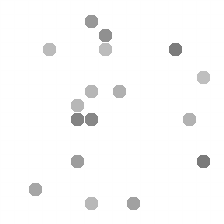
\includegraphics[width=0.4\textwidth]{images/sgw_random.png}}}
    \qquad
    \subfloat[\centering Tangram]{\fbox{
\includegraphics[width=0.4\textwidth]{images/tangram_random.png}}}
    \caption{The environments.}
    \label{fig:environments}
\end{figure}

\subsection{ShapeGridWorld}
\label{sec:sgw}
ShapeGridWorld is a pixel grid environment where the agent can draw on the grid by moving pixels around, either one or all of them at the same time.
This is reminiscent of the pin-board platform used in the free play study conducted by \citet{diggs} (\figref{fig:diggs}).
By setting the pixels in a specific layout, the agent can draw a variety of shapes on the grid.
This environment was adapted from the pixel grid environment used in the work by \citet{rair} with some modifications summarised in appendix \ref{sec:sgw-details}.

ShapeGridWorld was mostly used in the initial experiments but it later proved to promote noise in CLIP inferences which led to underwhelming results.
To work around the problems, the Tangram environment was developed.

\subsection{Tangram}
\label{sec:tangram}
Tangram is a traditional puzzle game consisting of a canvas and seven geometric shapes -- five right isosceles triangles (two large, one medium, and two small), one square, and one parallelogram, which conventionally have distinct colors.
These shapes can be rotated, flipped, and translated on the canvas, without overlapping.
Even though this is a very simple setup, these pieces can be arranged in very different configurations to create expressive abstract patterns.

The Tangram virtual environment was developed specifically for our experiments as it mitigated the problems discussed in sections \secref{sec:sparse-rewards} and \secref{sec:inference-noise}, and is a major contribution of our work.

We mostly configured the environment to correspond with the traditional Tangram game.
The shapes involved were the same, no overlap was allowed, and the shapes could be rotated, flipped, and translated.
Yet, we did experiments with colors to improve the performance of CLIP and also gave the agent the freedom to use a subset of the shapes to make its creations.
Please refer to appendix \ref{sec:tangram-details} for more technical details about this environment.

\section{Initial Tests with CLIP}
\label{sec:clip-custom}

% Talk about the initial tests with CLIP that were motivated by poor performance of CLIP on abstract images and sketches.
CLIP was trained on a large dataset of captioned natural images foraged from the internet.
While it generalizes well to many natural-image distributions and has proved to be a powerful zero-shot model for various tasks, it was not clear how well it would perform on sketches and abstract images. 

CLIP has been shown to not perform much better than chance on some tasks as they were not well represented in its pre-training dataset.
% For example, it only achieved 88\% accuracy on the handwritten digits of MNIST.
The authors of CLIP also noted that it is particularly poor on tasks for fine-grained classification such as differentiating models of cars, species of flowers, and variants of aircraft.
It also struggles with more abstract and systematic tasks such as counting the number of objects in an image.

Moreover, \cite{vlmrm}, from their experiments with CLIP as a source of goal-conditioned rewards, reported that CLIP rewards are only meaningful and well-shaped for environments that are photorealistic enough for the CLIP visual encoder to interpret correctly.
They found it crucial to add textures and shading to the images to make them more realistic for CLIP to perform well.

Influenced by these observations and caveats, we suspected that our environments, since they are not photorealistic, might also be out-of-distribution. 
Yet, we expected them to be simple enough for CLIP to interpret correctly.

Thus, before testing our reward function, we conducted a series of simple experiments on the inference capabilities of CLIP on ShapeGridWorld and Tangram.
At the same time, there were several hyperparameters in the environments and CLIP into which we took insights with these initial tests.

\subsection{CLIP on Sketches and ShapeGridWorld}
\label{sec:clip-sketches}

We first tested CLIP on sketches of simple shapes from the ImageNet-Sketch \cite{imagenet} dataset.

We also compared these results with renderings of these sketches on ShapeGridWorld grids of different resolutions by registering them (see \secref{sec:sgw-registration} for more details).

\begin{figure}[h]
    \centering
    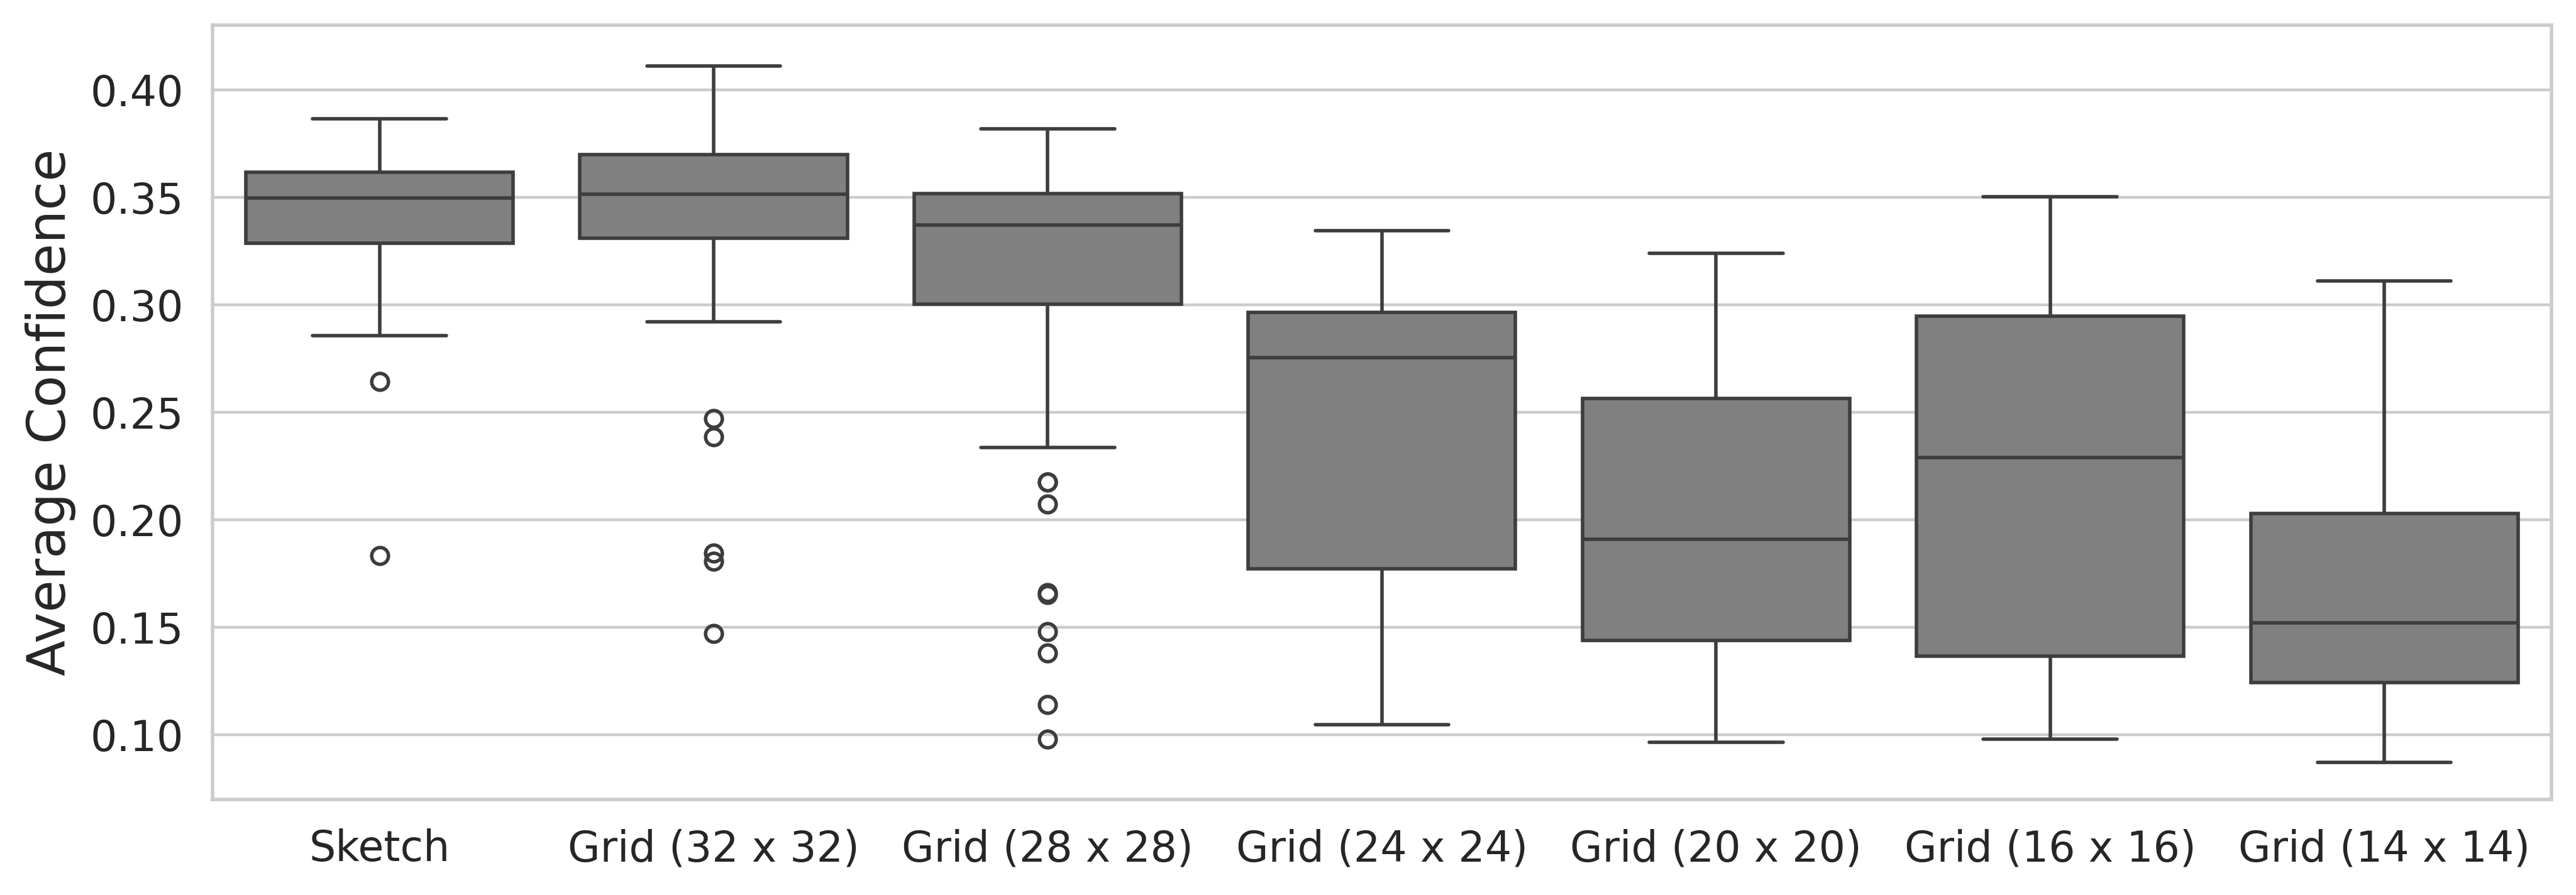
\includegraphics[width=\textwidth]{images/grid_comparison.png}
    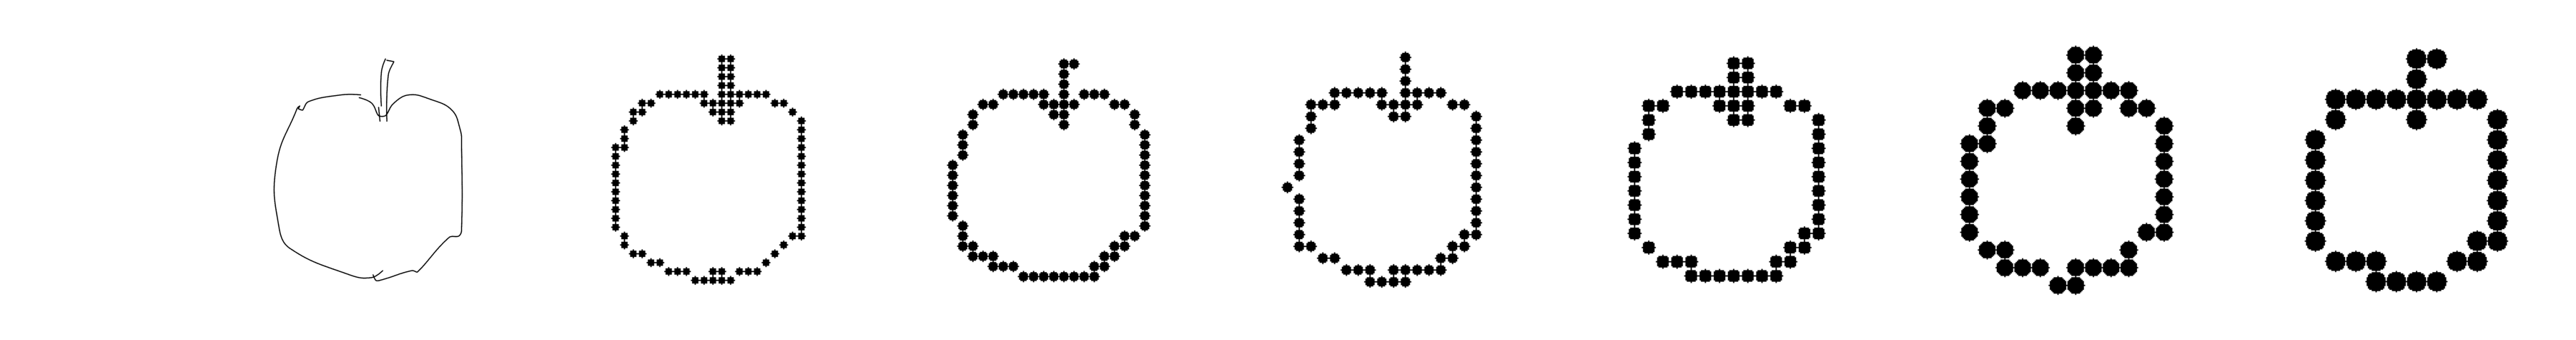
\includegraphics[width=\textwidth]{images/grid_comparison_images.png}
    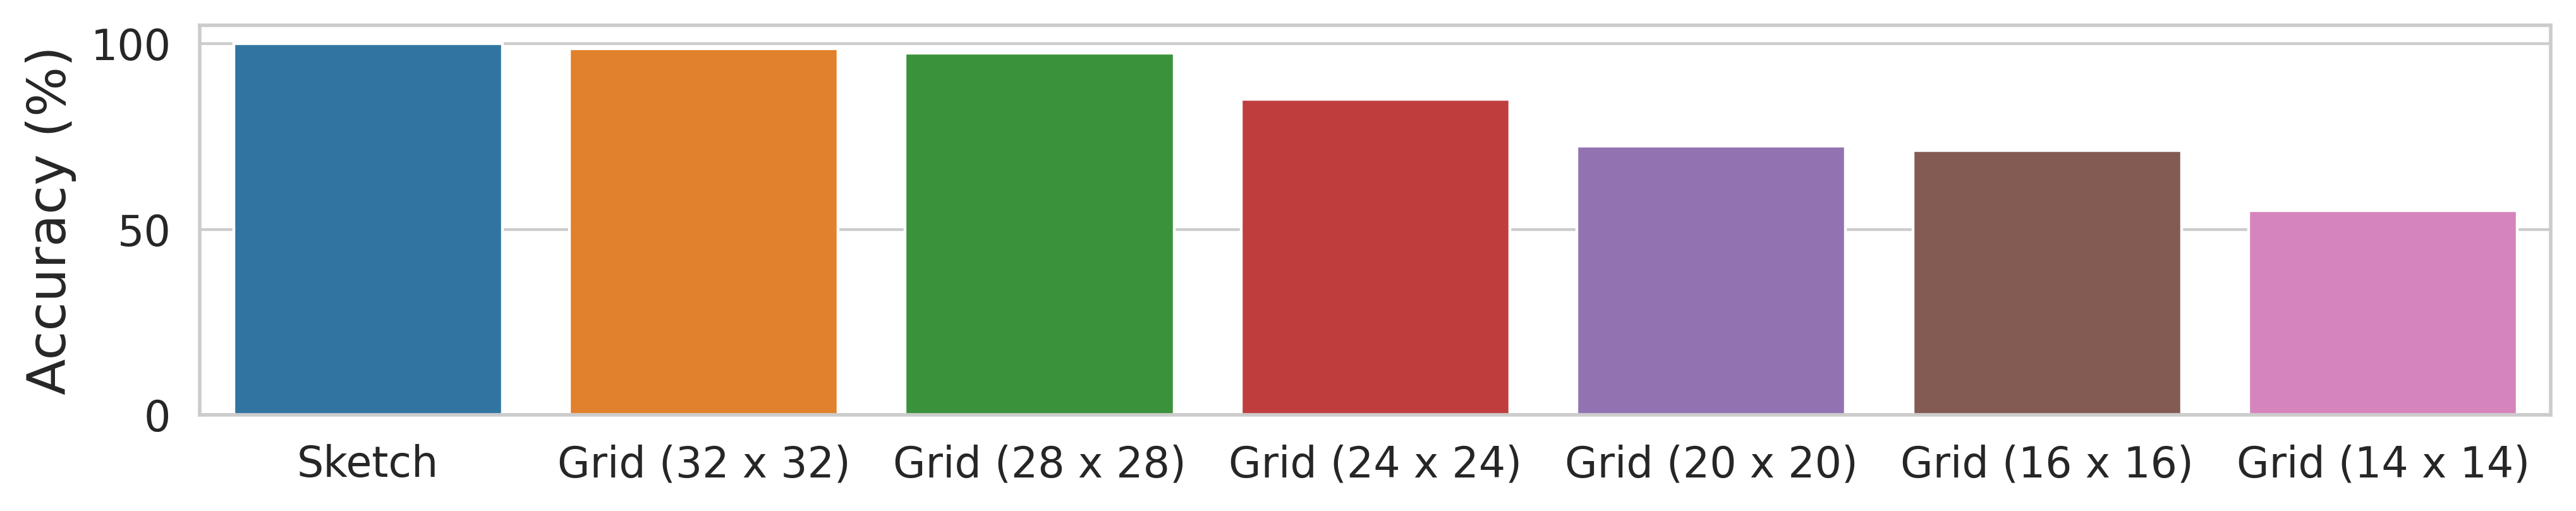
\includegraphics[width=\textwidth]{images/grid_comparison_accuracy.png}
    \caption{CLIP on sketches and ShapeGridWorld grids of different resolutions.}
    \label{fig:clip-sketches}
    % 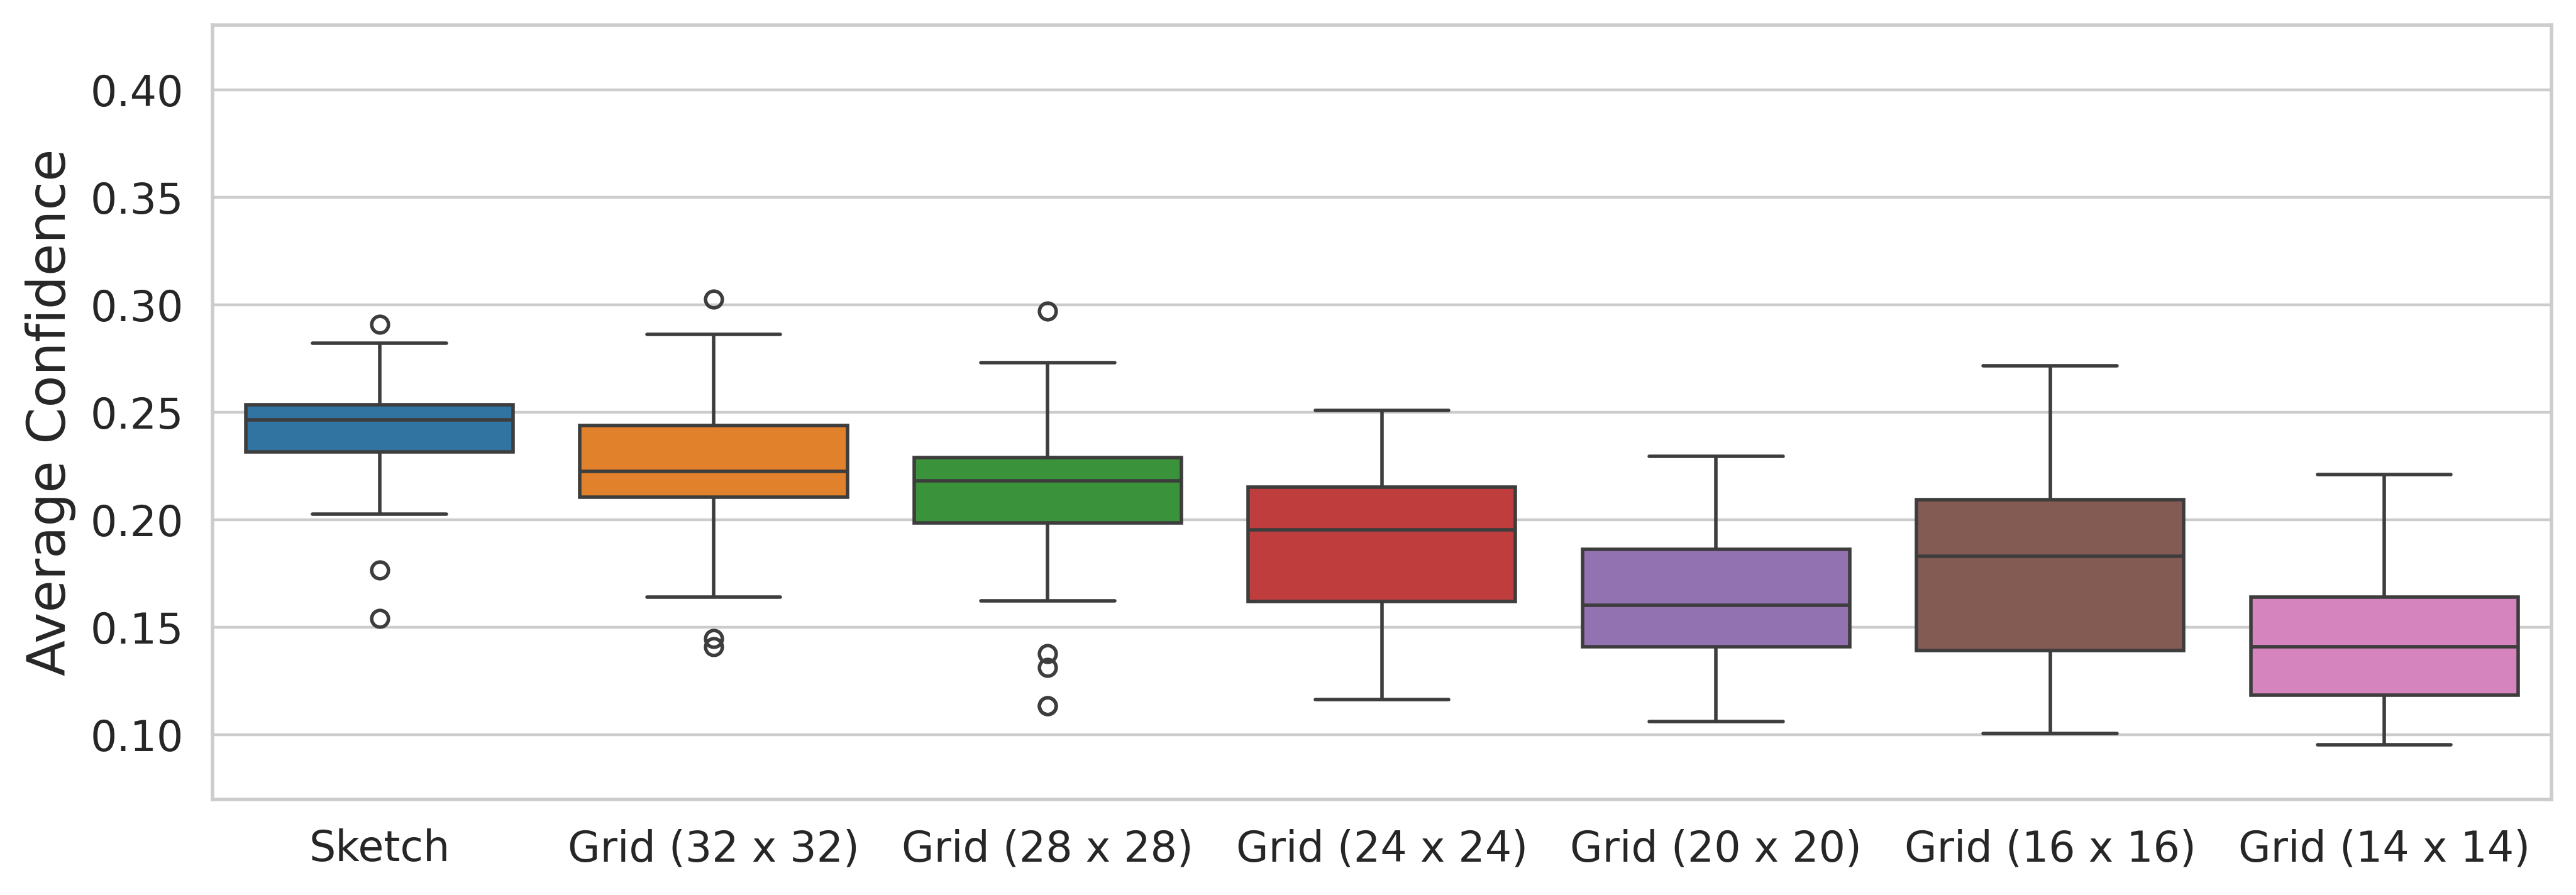
\includegraphics[width=\textwidth]{images/grid_comparison_generic.png}
    % \caption{CLIP on \emph{inverted} sketches and ShapeGridWorld grids of different resolutions.}
    % \label{fig:clip-sketches-inv}
\end{figure}

As an example, \figref{fig:clip-sketches} shows the comparative similarity of the embeddings of \(150\) sketches of apples (and their grid counterparts) to the label ``sketch of an apple'' using the CLIP variant \texttt{ViT-L/14}, as a probability.
The probabilities are calculated using the equation \eqref{eq:clip-dist}, with a higher temperature \(T = 1\), to show the trend.
The categories for this example are ``apple'', ``chair'', ``car'', ``flower'', ``pencil'', ``house'', ``tree'', ``fish'', ``star'', and ``bird''.
The middle row shows a sample of the images for each of the cases.
The bottom row shows the accuracy (percentage of correct predictions) for each of the cases.

We found that CLIP can recognize these sketches quite well.
As the grid became coarser, the confidence and accuracy of CLIP decreased significantly.
For very coarse grids, the accuracy is almost as bad as random guessing.
We also experimented with inverting the images and found that results were consistently slightly better with black-on-white sketches (shown here) than with white-on-black sketches.
We also noticed that using generic labels like ``fruit'' performed worse than using specific labels like ``apple''.

Additionally, we found that the bigger CLIP models performed significantly better on these tasks than the smaller ones which is in line with observations from other studies on VLMs as a source of rewards.
Furthermore, we tried the same experiments with different sets of categories, prefixes, and suffixes, but the results followed similar trends.
The later sections give more results for experiments on these hyperparameters.


\subsection{CLIP on Tangram}
\label{sec:clip-tangram}

Tangram has lesser degrees of freedom than ShapeGridWorld and it is more abstract but it still allows for rich creative expression.
To test if it would be a feasible environment for our study, we used some images of creations on Tangram from the internet and used CLIP as a zero-shot classifier as above to test its performance.

We again found it to be quite good at recognizing these creations with very high confidence.
\figref{fig:clip-tangram} shows a few examples.
Unlike ShapeGridWorld, we found no clear trend in the effect of color and inversions on the performance of CLIP.
More experiments on these hyperparameters are discussed in the later sections.

\begin{figure}[h]
    \centering
    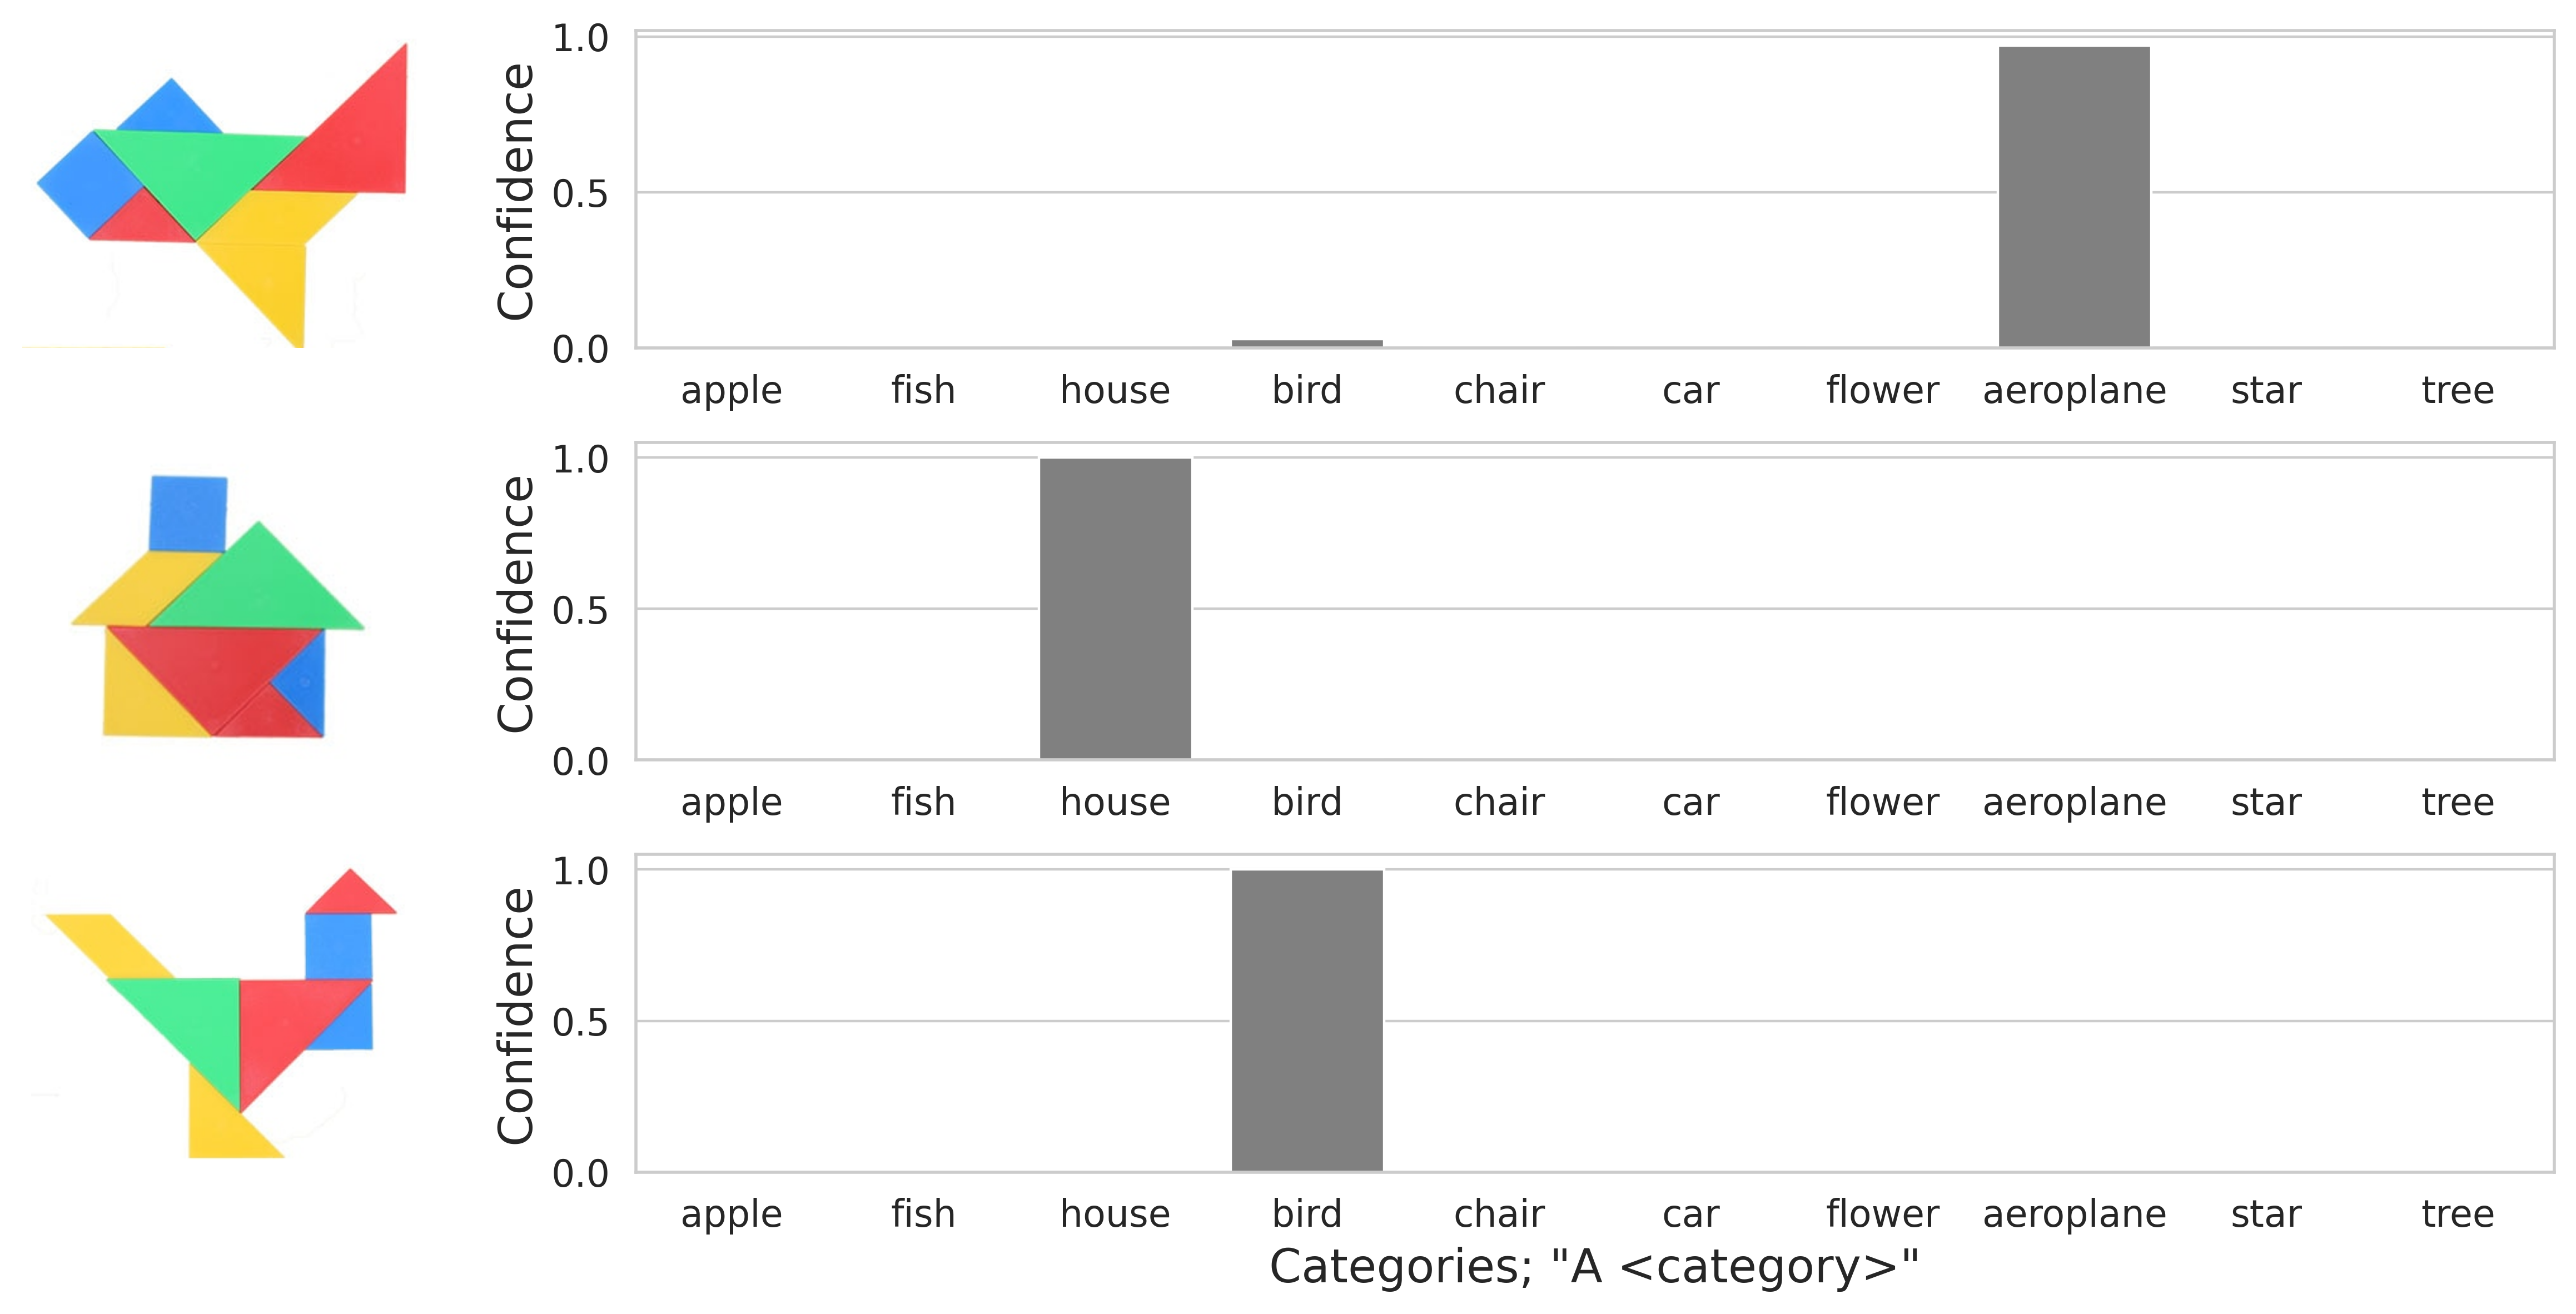
\includegraphics[width=\textwidth]{images/tangram_comparison.png}
    \caption{CLIP on a few simple Tangram creations.}
    \label{fig:clip-tangram}
\end{figure}


\section{Trajectory Analysis with Random Rollouts}
\label{sec:clip-problems}
% Problems with CLIP
Although we found that CLIP is quite good at recognizing these creations, we had to ensure that it would be a good source of rewards for our environments, or that the controller would be able to exploit it well to reach a sufficiently good local optimum.
To study the semantics entropy reward landscape, we conducted a series of experiments with random rollouts in the environments, i.e. starting from a meaningful creation, we perturbed the creation with randomly sampled actions and observed the effects on the reward.

These experiments showed that CLIP is quite susceptible to noise in its inferences, i.e. its probability distribution is very sensitive to small adjustments in the input image.
As a consequence of this, the reward is quite sparse, and more critically, there is a large semantic bias in not-so-meaningful images.
The sections below discuss these problems in detail.

\subsection{Sparse Rewards} % Sudden changes in rewards
\label{sec:sparse-rewards}

We observed that the inference of CLIP breaks suddenly with small changes in the image, i.e. its confidence in its classification changes very abruptly.
This results in a sparse semantics entropy reward landscape.
\figref{fig:sparse-rewards} illustrates this problem.
We destroy the image pixel by pixel using random actions left to right and see how CLIP's output changes.

\begin{figure}[h]
    \centering
    \missingfigure{Random rollouts in ShapeGridWorld and Tangram.}
    \caption{Random rollouts in ShapeGridWorld and Tangram.}
    \label{fig:sparse-rewards}
\end{figure}

Sparse rewards are a problem in reinforcement learning in general because underly a lack of continuous feedback. 
With only sporadic rewards, it becomes exceedingly difficult for an agent to gauge the values of actions to lead it to eventual rewards, i.e. credit assignment becomes difficult, which in turn leads to difficult and inefficient learning of action policies.

% If we imagine this scenario in reverse with an active controller, i.e. if the agent starts from the random image and tries to converge to a meaningful image by relying on the semantics entropy reward, it will have to take a series of actions that would sometimes lead to a reward and other times not.

Thus, a smooth and continuous reward is essential for effective learning.
Since we used the iCEM controller which is a gradient-free optimization algorithm and has proved to work well in sparse reward settings, we were able to circumvent this problem.

\subsection{Semantic Bias in Random Images} % Confidence in random images
\label{sec:inference-noise}
The other consequence of the noise in CLIP inference is that can sometimes confidently classify random images to a class, i.e. false positives, instead of having a flat distribution.
\figref{fig:semantic-bias-random} shows some instances of this problem where CLIP displayed high confidence in random images.

\begin{figure}[h]
    \centering
    \missingfigure{Large semantic bias in random images.}
    \caption{Large semantic bias in random images.}
    \label{fig:semantic-bias-random}
\end{figure}

This can also be interpreted as a jagged reward landscape with many local optima.
This noisy reward signal can lead the agent to be stuck in local optima (with a rather meaningless creation that it erroneously finds confident), or inhibit it from reaching a good optimum.

\subsubsection{Class Preference in CLIP}
Another problem we faced related to the problem of semantic bias in random images was that of class imbalance.
There were some classes that CLIP was usually confident in than others.

\begin{figure}[h]
    \centering
    \missingfigure{Class preference in CLIP.}
    \caption{Class preference in CLIP.}
    \label{fig:class-preference}
\end{figure}

\section{Improving CLIP Rewards}
\label{sec:improving-rewards}

The two problems, sparse rewards and semantic bias in random images are not independent. They have the same underlying cause -- noisy CLIP inference, yet there's a non-trivial anticorrelation between reward sparseness and noise.
That is, increasing reward density involves increasing confidence in imperfect/partial creations which also increases noise.

We experimented with several methods to improve the rewards from CLIP.
This section discusses the strategies we used to tackle these problems and improve the rewards.

\subsection{Effect of the Number of Creative Possibilities}
\label{sec:clip-categories}
We found that the number of creative possibilities in the environment can also affect the performance of CLIP.
Too few categories can promote semantic bias and class preference in random images, but too many categories can exacerbate the problem of sparse rewards.
We found that the best results were obtained with a moderate number of categories, i.e. around \(10 \sim 15\).
This greatly helped in reducing the class preference in CLIP.

\begin{figure}[h]
    \centering
    \missingfigure{Effect of the number of categories on CLIP rewards.}
    \caption{Effect of the number of categories on CLIP rewards.}
    \label{fig:clip-categories}
\end{figure}

\subsection{Adversarial Performance}
\label{sec:adversarial-performance}
To tackle the problem of semantic bias in random images, we collected samples of these image observations from our experiments, called \emph{adversarial observations}, and tried to pick regularization hyperparameters of the semantics reward function that would make CLIP less confident in these images while maintaining its inference for the semantically expressive images.

\figref{fig:adversarial-images} shows the results of our analysis.
\begin{figure}[h]
    \centering
    \missingfigure{Adversarial images.}
    \caption{Adversarial images.}
    \label{fig:adversarial-images}
\end{figure}



\subsection{Post-hoc Analysis on Rollouts with Closeness Costs}
\label{sec:closeness-rollouts}
% closeness_reward_scale
% closeness_reward_threshold
The choice of the iCEM controller hyperparameters and the environment configuration was crucial to ensure that an agent was able to achieve a goal under sparse rewards in our environment.
These hyperparameters and configurations were dependent on each other so we needed to optimize them together.
Please refer to appendix \ref{sec:icem-hyperparameters} for more details about the iCEM controller.

For example, for the Tangram environment, the size of the grid together with the step size governs the controller's planning horizon.
For a small discrete grid or a large discrete grid with a large enough step size, the planning horizon does not need to be very high, but if the step size is too small for the grid size, the planning horizon needs to be high.
The step size is also related to the object persistency used in the environment.

Given the high computation resources and time required to run simulations with the semantics entropy reward, it was infeasible to do even an exhaustive search over all the hyperparameters.
Thus, we instead used an alternative reward function to analyze the effect of the hyperparameters.
We called this ersatz reward function the \emph{closeness reward}.

A closeness reward is defined in the context of a fixed target creation in the environment, and its function is given as the negative of a distance function between the current creation and the target creation in the state space of the environment.

We used two different formulations of the distance function, which we called the \emph{dense closeness cost} and \emph{sparse-incremental closeness cost}.
The \emph{dense closeness cost} is formulated as the \(L^2\) distance between the current and target creations and the \emph{sparse incremental closeness cost} is formulated as the dimension-wise thresholded \(L^1\) distance between the current and target creations. It is given by 
\begin{equation}
    \label{eq:closeness-reward-sparse}
    d(\bfi, \bft) = \sum_{k \in n_s} \bm{1}_\varepsilon(\bfi_k - \bft_k),
\end{equation}
where \(\bfi, \bft \in \cS\) are the current and target creations respectively, \(\varepsilon\) is a small threshold, and \(\bm{1}_\varepsilon\) is the indicator function such that \(\bm{1}_\varepsilon(x) = 1\) if \(|x| > \varepsilon\) and \(0\) otherwise.

Using the closeness reward/cost formulations, we performed a grid search over the many hyperparameters of the iCEM controller and the environment to find the best combination.

The results for the \emph{sparse incremental closeness cost} on the Tangram environment are shown in \figref{fig:closeness-rollouts}.

To rank the rollouts generated through 

\begin{figure}[h]
    \centering
    \missingfigure{Closeness rollouts in Tangram.}
    \caption{Closeness rollouts in Tangram.}
    \label{fig:closeness-rollouts}
\end{figure}

% Manual ranking and entropy ranking

\subsubsection{Tuning Environment Parameters}
\label{sec:env-hyperparameters}
% render_kwargs.invert
% render_kwargs.color


\label{sec:sgw-hyperparameters}
% width
% x_step
% render_delta
% object_persistency
% max_dist
% control
% control_boundaries


\label{sec:tangram-hyperparameters}
% flip
% rotate
% x_size
% r_size
% x_step
% object_persistency
% max_dist
% control
% control_boundaries
% staging_boundaries


\subsubsection{Tuning Controller Hyperparameters}
\label{sec:icem-hyperparameters}
% action_sampler_params.opt_iterations
% action_sampler_params.init_std
% action_sampler_params.elites_size
% num_simulated_trajectories
% horizon
% cost_along_trajectory
% discount_along_trajectory


\subsection{Effect of Target Baseline Regularization}
\label{sec:reg-alpha}
% semantics_alpha_target


\subsection{Effect of Image Baseline Regularization}
\label{sec:reg-beta}
% semantics_beta_image


\subsection{Effect of Temperature}
\label{sec:reg-temperature}
% semantics_model_temperature


\subsection{Effect of Changing Prefix and Suffix}
\label{sec:prefix-suffix}
% label_prefix
% label_suffix


\subsection{Effect of Adding Post-Suffix}
\label{sec:post-suffix}
% Jibberish and adding concepts in post-suffix (WaffleCLIP)
% \cite{waffleclip} found that the exact structure of the phrase, and even tailing it a random string of jibberish, can affect the reward.


\subsection{Effect of Negative Embeddings}
\label{sec:negative-embeddings}


\subsection{Effect of Image Operations}
\label{sec:image-operations}
% Shearing and Hatching


\subsection{Entropy Regularization}
\label{sec:entropy-regularization}
Another promising way to make the reward landscape of CLIP smoother is to fine-tune it with an additional entropy regularization loss over its output.
This is given by,
\begin{equation}
    \label{eq:entropy-regularization}
    L(\bmi, \bml) = L_{\iota}(\bmi, \bml) \underbrace{- \sum_{\bfi_k \in \bmi}\sum_{\bfl_j \in \bml} p(\bfl_j; \bfi_k, \bml) \log p(\bfl_j; \bfi_k, \bml)}_{\text{Entropy Regularization}},\\
\end{equation}
where \(L_{\iota}\) is the contrastive cosine-similarity loss used to train CLIP and \(p(\bfi_k, \bml)\) is the classification probability distribution of image \(\bfi_k\) over the labels \(\bml\) predicted by CLIP.

We experimented with this regularization method on a toy convolutional neural network (CNN) for classifying handwritten digits, which we called \emph{Flatnet}.
We found it to be quite effective in smoothing the reward landscape.
Both our problems from \secref{sec:clip-problems} were relieved -- the reward trajectory was smoother and we observed less semantic bias in random images.

Yet, we did not use it to fine-tune CLIP to limit the scope of the project given the limited time.
The results of this analysis can be found in appendix \ref{sec:flatnet}.

\newpage
\section{Simulations}
\label{sec:simulations}
% Manual ranking and entropy ranking


\subsection{Effect of RaIR}
\label{sec:effect-rair}
% compression_precision
% 1 / semantics_reward_scale


\subsection{Partial Completions on ShapeGridWorld}
\label{sec:partial-completion}
